Le modalità di sviluppo e la scelta degli strumenti, hanno premesso di creare
un'applicazione modulare. Modelli e procedure sono state più volte modificate
nel corso della progettazione e implementazione. La scelta di usare un database
non relazionale, di aderire al pattern architetturale \acf{MVC} e al promise
pattern ha permesso di elaborare un'applicazione solida e facilmente
modificabile. 

Il modello stesso dei dati salvato nel database
CouchDB è stato più volte cambiato, aggiungendo e modificando proprietà
dell'oggetto senza riscontrare difficoltà nella definizione dei tipi di dati.
Diversamente sarebbe stato se avessi utilizzato un database relazionale. CouchDB
si è dimostrato una scelta valida anche per quanto riguarda la sincronizzazione
dei dati. Trovandosi di fronte a una situzione in cui più host dovevano
dialogare fra di loro, i metodi, facilmente configurabili, messi a disposizione
dal database hanno agevolato il passaggio di dati fra sede centrale e filiali.

La struttura aderente al pattern \ac{MVC} a promise pattern, invece, permette di
inserire nuove azioni che vanno a dialogare con i modelli. Ogni funzione viene
implementata in modo indipendente dalle altre, in quanto lo stato di una
promessa può essere fulfilled, restituendo il contenuto, oppure rejected.
Funzioni concatenate fra loro devono solo gestire i due casi appena citati.
Saranno implementate nuove funzioni per gestire il login per gli amministratori
al momento della visualizzazione dei grafici.
Questa sezione verrà implementata utilizzando un proprio framework \ac{PHP} in
fase di sviluppo che gestirà la fase di autenticazione, implementazione di \ac{ACL} e
la sicurezza dei dati. Ulteriori funzionalità verranno aggiunta per quando
riguarda l'analisi dei dati, permettendo di confrontare fra loro più sedi.
L'utilizzo di richieste \acf{AJAX} parallele consente già di
ottenere tutti i dati necessari per la composizione di nuovi grafici.

L'applicazione ha soddisfatto le attese del cliente committente e allo stato
attuale è installata in versione di prova in alcune sedi. Si è cercato inoltre
di implementare il codice in modo da lasciare ampio spazio alle customizzazioni,
così da ottenere un modello valido anche per altre utilizzazioni future. 
\newpage
\section{screenshot}
  \begin{figure}[!h]
    \begin{center}
      
\includegraphics[scale=0.30]{icons/screen_intro.png}
      \caption{Schermata introduttiva}
      \label{fig:screen_intro}
    \end{center}
  \end{figure}
  \begin{figure}[!h]
    \begin{center}
      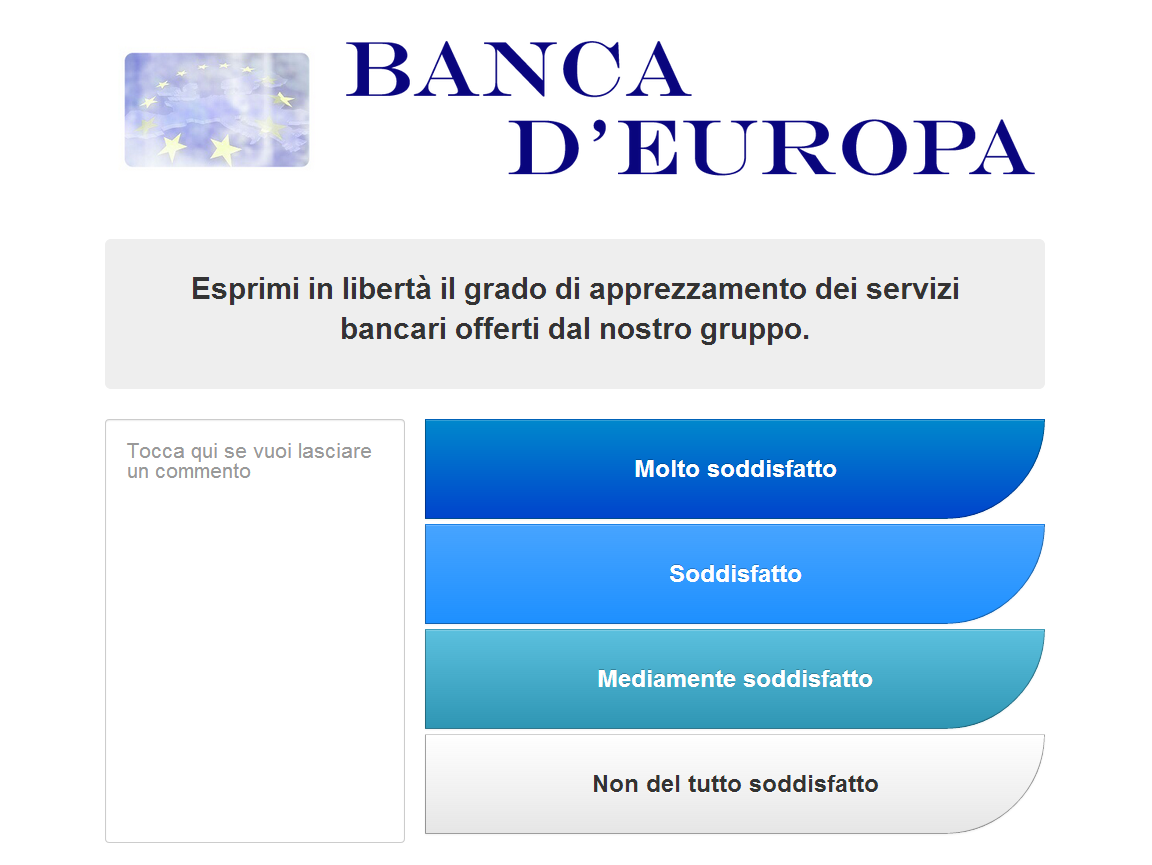
\includegraphics[scale=0.30]{icons/screen_voting.png}
      \caption{Scelta del livello di soddisfazione}
      \label{fig:screen_voting}
    \end{center}
  \end{figure}
  \begin{figure}[!h]
    \begin{center}
      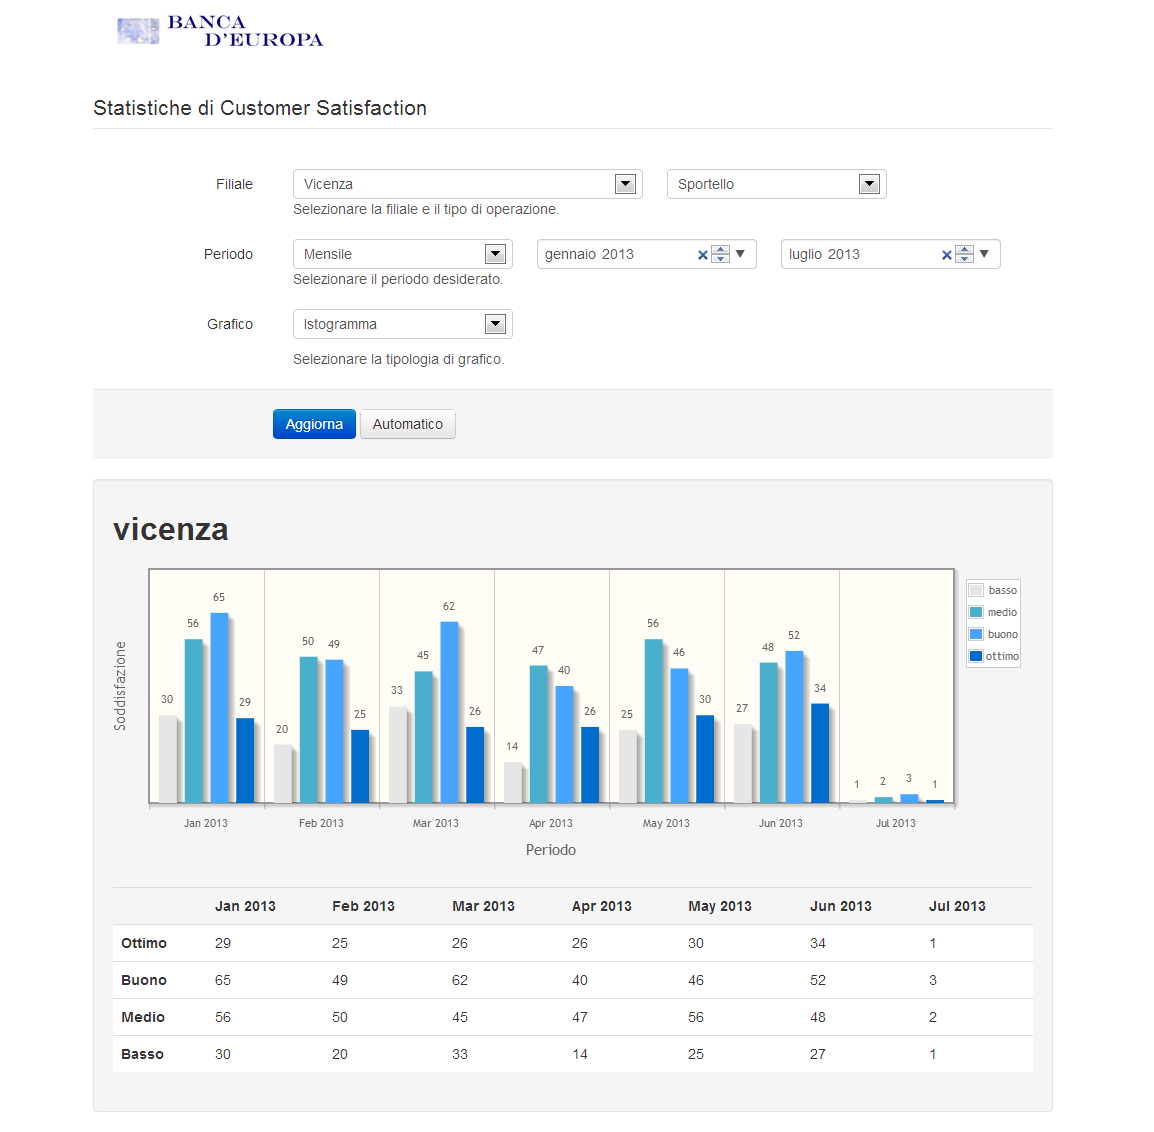
\includegraphics[scale=0.35]{icons/screen_graph.png}
      \caption{Generazione dei grafici}
      \label{fig:screen_graph}
    \end{center}
  \end{figure}
